\section{Pathway Browser Implementation}
\label{sect:maw_implementation}

\mawappp pathway visualization is relatively simple in terms of its data model;
the \pathcasemaw web service provides all information in terms of graphical
objects such as nodes and edges. \mawapp doesn't need to make any rendering
decisions about an attribute like a node's color based on, for example, a
metabolite's role in a reaction. It simply renders exactly what \pathcasemaw
instructs.

The pathway visualization system was the first part of the project to be
implemented. Its limited scope made it easy to design a graph renderer that is
decoupled from the specific kind of data it displays. Although the design did
have to be modified to be used in \keggapp, the changes were not significant,
and eventually the two applications may share the same code for this component.

Section \ref{sect:smda_arch_overview} describes the general architecture of
\mawappp pathway visualizer. Section \ref{sect:smda_viz_data} describes in
detail the process of loading a graph into memory from its \pathcasemaw
representation. Finally, section \ref{sect:smda_rendering} describes how the
model objects are rendered to the screen.

\subsection{Architecture Overview}
\label{sect:smda_arch_overview}

\begin{figure}[p]
    \center{
        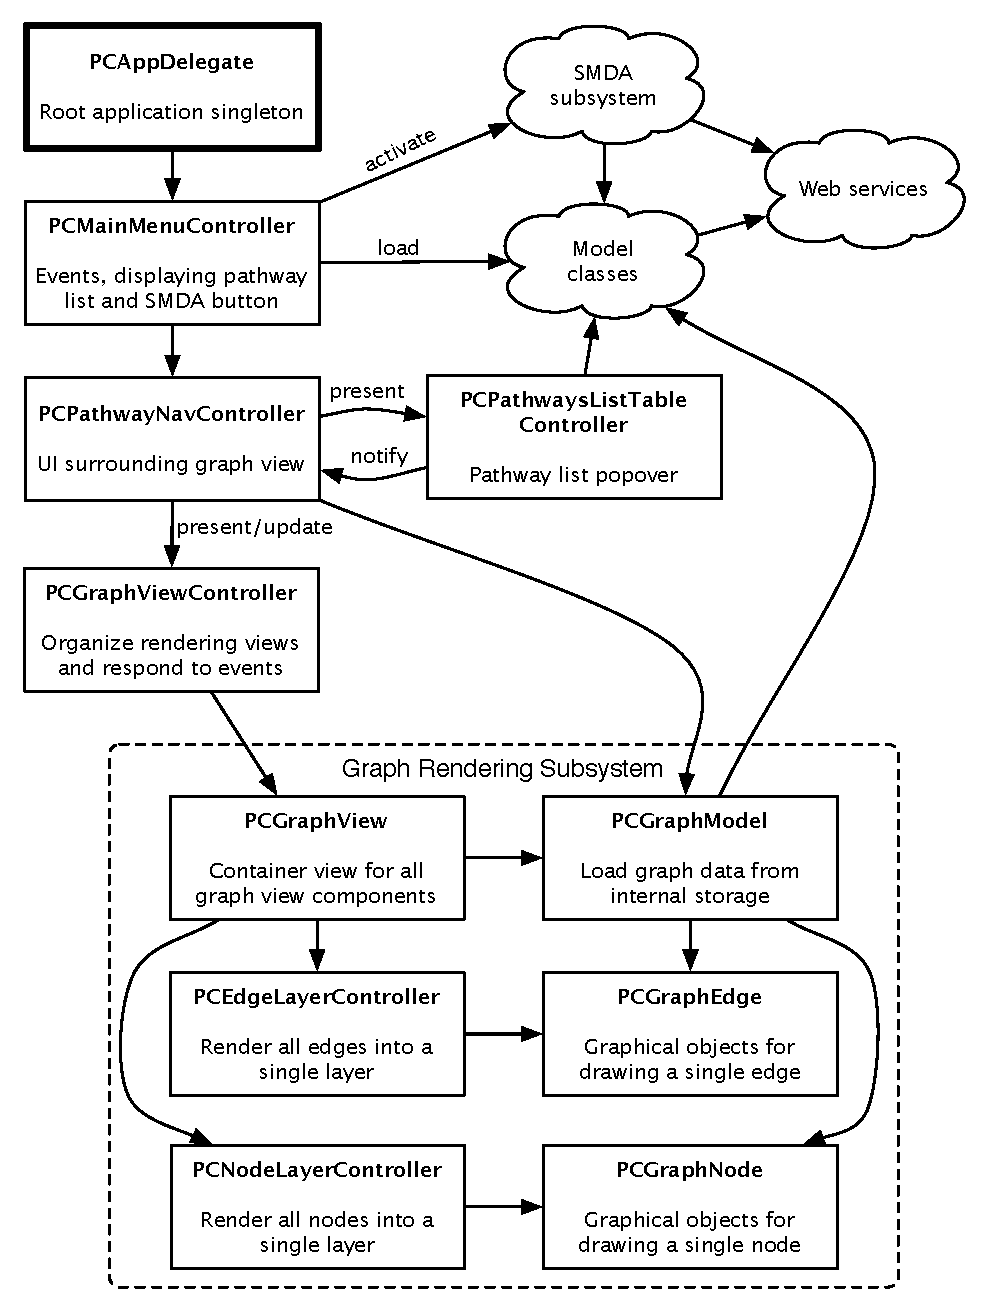
\includegraphics[width=\textwidth]{maw/figures/components.pdf}}
    \caption{\label{fig:maw_components} Components of the architecture. See
    \ref{sect:smda_arch_overview} for more information about this diagram.}
\end{figure}

Figure \ref{fig:maw_components} shows a high-level representation of the
relationships between the most important objects in \mawapp. Most of the classes
discussed here and shown in the figure fall into the category of model, view, or
controller. For more information about Model-View-Controller design, see section
\ref{sect:cocoa_mvc}.

An application-level singleton, \texttt{PCAppDelegate}, handles
application-level delegate methods and notifications from the system. Another
singleton, \texttt{PCMainMenuViewController}, displays the home screen,
including the list of pathways and button to enter SMDA. It also initiates the
download of the model objects if they require an update. This relationship is
represented by the \emph{activates} and \emph{loads} arrows in figure
\ref{fig:maw_components}.

When an item in the list of pathways is tapped, a new view is shown, controlled
by \texttt{PCPathwayNavController}. This view controller object controls the
toolbar and a content area that can contain any view and corresponding view
controller. See the screenshot in figure \ref{fig:maw_screenshot_pathway} to see
how this toolbar is displayed to the user.

The content area is controlled by \texttt{PCGraphViewController}. This view
controller object controls a \texttt{PCGraphView} which renders the pathway
visualization based on a \texttt{PCGraphModel} and sends notifications back to
the \texttt{PCGraphViewController} if an event occurs (e.g. a node being tapped).

As shown in figure \ref{fig:maw_screenshot_pathway_list_popover}, the
``Pathways'' button in the toolbar controlled by \texttt{PCPathwayNavController}
displays a list of pathways that may be visualized. The loading and display of
this list is handled by \texttt{PCPathwayListTableController}, which loads
pathway model objects (\ref{sect:smda_data_model}) and converts them
to a list to be displayed by a table view (\ref{sect:ipad_views}). When a table
view row is selected, the \texttt{PCPathwayListTableController} sends a
notification back to the \texttt{PCPathwayNavController}, which replaces its
content area with a \texttt{PCGraphViewController} representing the new pathway
to be displayed.

The control flow of \texttt{PCPathwayNavController} at runtime is shown in
figure \ref{fig:maw_controlflow}. This object has no event loop of its own; its
functionality is invoked by the application event loop provided by the Cocoa
framework. When the ``Pathways'' button is pressed, it creates a
\texttt{PCPathwayListTableController} which presents a popover containing a
table view, loads the list of pathways, populates the table view, and sends
control back to the event loop. When a row is tapped in this table view, the
\texttt{PCPathwayListTableController} sends a notification back to the
\texttt{PCPathwayNavController}, which hides the popover, loads the new pathway
visualization, and displays it.

\begin{figure}[thbp]
    \center{
        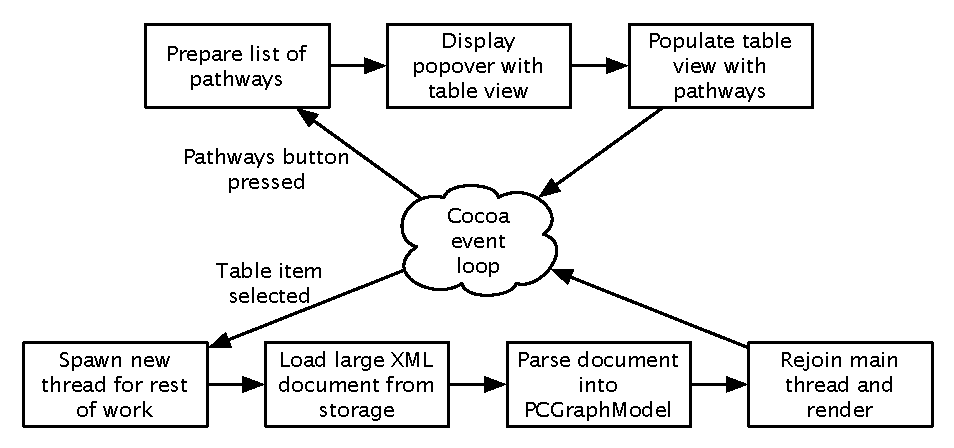
\includegraphics[width=5in]{maw/figures/controlflow.pdf}}
    \caption{\label{fig:maw_controlflow} Control flow of
    \texttt{PCPathwayNavController}}
\end{figure}

\texttt{PCGraphViewController} and \texttt{PCGraphModel} are the high level
interface to the pathway visualization subsystem. \texttt{PCGraphModel} holds
collections (hash tables) of \texttt{PCGraphNode} and \texttt{PCGraphEdge}
objects. These objects represent the visual properties of each node and edge in
the graph, including location, color, shape, label text, and label position. The
\texttt{PCGraphViewController} and its helper objects render the graph
represented by the \texttt{PCGraphModel} to a scroll view
that the user can navigate by touch (\ref{sect:ipad_views}). 

\subsection{Loading Graph Data}
\label{sect:smda_viz_data}

This section describes how data is obtained from the \pathcasemaw server and
converted into objects that can be rendered on the iPad.

\subsubsection{The \texttt{GetPathwayData} Web Service}

The pathway visualization data (graph data) is provided by the \pathcasemaw web
service \texttt{GetPathwayData}
\footnote{\url{http://nashua.case.edu/PathwaysMAWService/PathwaysService.asmx?op=GetPathwayData}}.
Rather than call the web service when the user requests to view a pathway, the
web service responses for \emph{all} pathways are included with the application
itself in the form of text files. Each text file contains the HTTP response to a
web request for the graph data for one pathway.

The graph data changes very rarely, so including the data with the application
lets the user use visualizations without an internet connection, without waiting
for a web request to complete, and without major penalties for being out of date
with the \pathcasemaw database.

\subsubsection{Graph Model}

A pathway visualization (graph) consists of nodes (\texttt{PCGraphNode} and
edges (\texttt{PCGraphEdge}). These nodes and edges are collected in a
\texttt{PCGraphModel} which represents the entire visualization.

Node and edge objects have two public interfaces. One is the \emph{construction}
interface, used by the code that builds the model. The other is the
\emph{rendering} interface, which the rest of the rendering system uses to draw
the objects in Core Animation (\ref{sect:core_animation}). These interfaces
overlap slightly for basic attributes such as position or source and target
node. Tables \ref{fig:smda_node_interface} and \ref{fig:smda_edge_interface}
show the relevant attributes and functions for these interfaces.

If a node or edge is \emph{highlighted}, it is drawn with a green glow beneath
it. This is used in the SMDA tool part of the application to highlight
differences between graphs. Figure \ref{fig:smda_results_highlight} demonstrates
this behavior.

\begin{table}[htbp]
\centering
\begin{tabular}{ p{1.5in} p{3in} p{0.3in} p{0.3in}}
    Attribute & Description & Const & Rend \\ \hline
    \hline \multicolumn{4}{c}{Attributes} \\ \hline

    identifier  & Unique key  & Y & Y \\
    fullName  & Full name to be displayed in popover when tapped & Y & Y \\
    label  & Label to be displayed in the main visualization & Y & Y \\
    size  & Size & Y & Y \\
    position  & Position & Y & Y \\

    fill  & Fill color of the shape & Y & Y \\
    outline  & Outline color of the shape & Y & Y \\
    labelColor  & Color of the label & Y & Y \\
    labelAnchor  & Location of the label relative to the shape & Y & Y \\

    isGroup  & Node is a box around other nodes (e.g. a compartment) & Y & Y \\

    type & Which shape (e.g. rectangle, circle) to draw
    & Y & Y \\

    highlighted & Node should be drawn with a highlight glow
    & Y & Y \\

    hierarchicalIdentifier  & Unique key including parent compartments
    & Y & N \\
    isComplete & Used during node expression parsing
    & Y & N \\

    labelLayer  & \texttt{CALayer} that renders the node's text label
    & N & Y \\

    highlightNodeLayer  & \texttt{CALayer} that renders the node's highlight
    glow
    & N & Y \\

    \hline \multicolumn{4}{c}{Methods} \\ \hline

    initWithTokenizer: & Create rendering objects
    & Y & N \\

    drawInContext: & Draw this node
    & N & Y \\
\end{tabular}
    \caption{Construction and rendering interfaces for \texttt{PCGraphNode}}
    \label{fig:smda_node_interface}
\end{table}

\begin{table}[htbp]
\centering
\begin{tabular}{ p{1.5in} p{3in} p{0.3in} p{0.3in}}
    Attribute & Description & Const & Rend \\ \hline
    \hline \multicolumn{4}{c}{Attributes} \\ \hline

    identifier & Unique key  & Y & Y \\
    fill & Color of the line & Y & Y \\
    width & Width of the line & Y & Y \\
    highlighted & Draw with a highlight glow & Y & Y \\

    source & Node to draw from & Y & Y \\
    target & Node to draw to & Y & Y \\

    \hline \multicolumn{4}{c}{Methods} \\ \hline

    initDrawingWithOffset: hasPartner: & Create rendering objects
    & Y & N \\

    drawInContext: & Draw this edge
    & N & Y \\

    drawHighlightInContext: & Draw this edge's highlight glow
    & N & Y \\
\end{tabular}
    \caption{Construction and rendering interfaces for \texttt{PCGraphEdge}}
    \label{fig:smda_edge_interface}
\end{table}

\subsubsection{Parsing Graph Data}

Figure \ref{fig:maw_viz_data} shows the complete pipeline for converting data
from \texttt{GetPathwayData}'s response format to the graph model described in the
previous section. 

\texttt{GetPathwayData}'s responses come in two parts, separated by the string
``\texttt{\#\#\#}''. The first part is a GML (Graph Modeling Language) string
\cite{gml}. The second part is XML containing extra information about some
nodes. \mawapp discards the second part.

The GML is generated by the yFiles library \cite{yfiles}. Here is an informal
summary of the subset of GML generated by \texttt{GetPathwayData}:

\begin{objc}
Creator "yFiles"
Version "2.5.0.3"
graph
[
    hierarchic  1
    label       ""
    directed    1
    node
    [
        id  0
        label   "Short label"
        graphics
        [
            x       796.6842041015625
            y       78.52631378173828
            w       20.0
            h       20.0
            type    "ellipse"
            fill    "#FFFF00"
            outline "#000000"
        ]
        LabelGraphics
        [
            text            "Short label" // label is defined twice
            fontSize        10
            fontName        "Arial"
            autoSizePolicy  "node_width"
            anchor          "ne"
        ]
        idMap   "Long label displayed when node is tapped"
        typeMap 1
        gid     28
    ] // repeat for each node
    edge
    [
        source  27 // These refer to node 'id's
        target  23
        graphics
        [
            type        "arc"
            fill        "#000000"
            sourceArrow "delta"
            targetArrow "standard"
            arcType     "fixedRatio"
            arcHeight   18.763839721679688
            arcRatio    1.0
            Line
            [
                point
                [
                    x   1026.7894287109375
                    y   271.52630615234375
                ]
                point
                [
                    x   1052.68408203125
                    y   238.5131378173828
                ]
                point
                [
                    x   1094.631591796875
                    y   239.42105102539062
                ]
            ]
        ]
    ] // repeat for each edge
]
\end{objc}

This simple data format is tokenized using the tokenizer functionality of the
open source library ParseKit \cite{parsekit}, which handles string escapes and
other common tokenizing tasks. The subset of GML used by \pathcasemaw has a
regular grammar, so no complex parsing algorithm is required.  The only real
complexity is introduce by the fact that a single node or edge may appear more
than once in the document with different subsets of attributes filled in. The
parsing algorithm must therefore be careful to update a node or edge if it has
already been parsed, rather than overwriting it with an entirely new value.

\texttt{PCGraphModel} is the object that handles the parsing of this data
format. It loops over a token stream from ParseKit looking for the keyword
\texttt{node} or \texttt{edge}. If it is \texttt{node}, then a
\texttt{PCGraphNode} is created to parse the node expression. If it is a
\texttt{edge}, then a \texttt{PCGraphEdge} is created to parse the edge
expression. The resulting nodes and edges are either stored in memory or update
an existing node or edge object with the same identifier that already exists.

Once all the data has been parsed, the nodes' and edges' rendering objects are
initialized.

\begin{figure}[thbp]
    \center{
        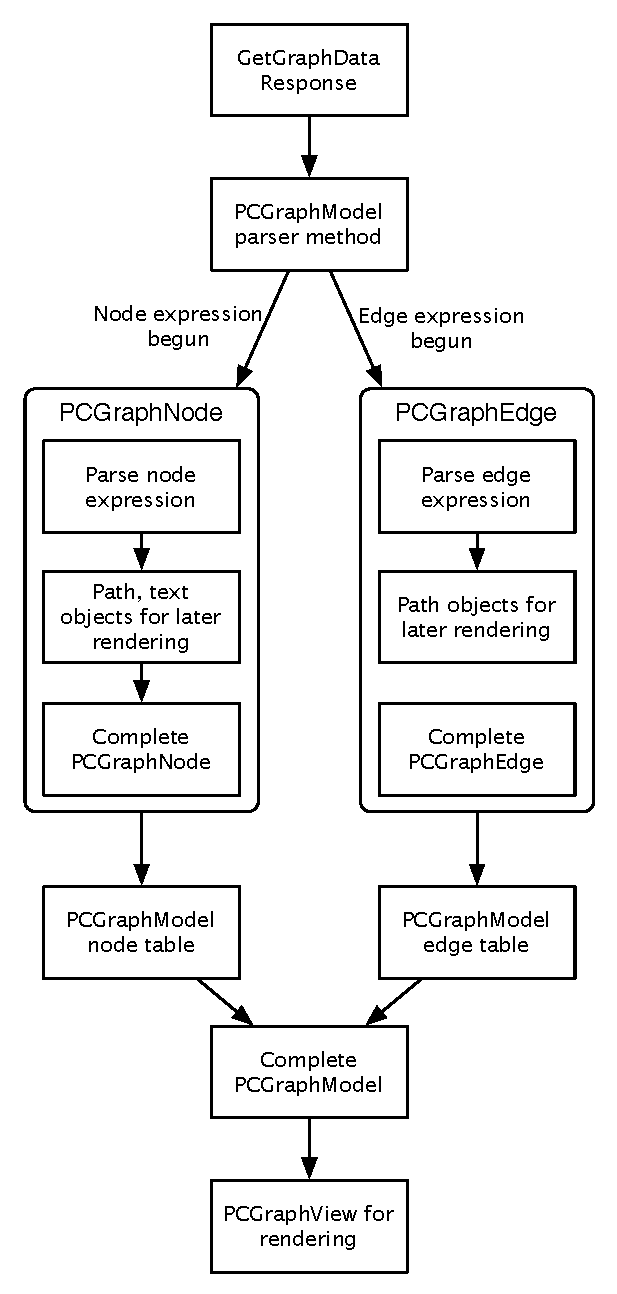
\includegraphics[width=3.5in]{maw/figures/dataflow.pdf}}
    \caption{\label{fig:maw_viz_data} Data flow from \pathcasemaw representation
    to final display format. See section \ref{sect:smda_viz_data} for more
    information about this diagram.}
\end{figure}

\subsection{Rendering}
\label{sect:smda_rendering}

After \texttt{PCGraphModel} has parsed all of the data, the graph is ready for
rendering by a \texttt{PCGraphView}. \texttt{PCGraphView} uses a Core Animation
layer hierarchy (see section \ref{sect:core_animation}) to draw the graph
efficiently. There are four layers in a \texttt{PCGraphView}. From top to
bottom:

\begin{enumerate}

    \item \textbf{Text layer} for drawing node labels. This layer contains
        one sublayer for each node that renders the text for its label.

    \item \textbf{Node layer} for drawing node shapes. This layer is drawn by
        calling \texttt{drawInContext:} on each node object.

    \item \textbf{Edge layer} for drawing edges. This layer is drawn by calling
        \texttt{drawInContext:} on each edge object. Each edge may optionally
        render a highlight glow before rendering the actual edge.

    \item \textbf{Node highlight layer} for drawing node highlight shapes. This
        layer contains one sublayer for each node that renders its highlight
        glow. These sublayers are invisible unless the node is marked as
        highlighted.

\end{enumerate}

Once these layers are rendered, they are drawn to the screen by a scroll view
(see section \ref{sect:ipad_views}) which takes care of translating and scaling
them in response to user interaction.
